\begin{center}
	\begin{tabular}{M{9.25cm}M{8.75cm}}
		\textbf{TRUNG TÂM MANABIE}& \textbf{ÔN TẬP KIỂM TRA CUỐI HỌC KÌ I}\\
		\textbf{MÃ ĐỀ: 001}& \textbf{Bài thi môn: VẬT LÝ 11}\\
		\textit{(Đề thi có 04 trang)}& \textit{Thời gian làm bài: 50 phút, không kể phát đề}
		
		\noindent\rule{4cm}{0.8pt} \\
	\end{tabular}
\end{center}
\setcounter{section}{0}
\section{Câu trắc nghiệm nhiều phương án lựa chọn}
\textit{Thí sinh trả lời từ câu 1 đến câu 18. Mỗi câu hỏi thí sinh chọn một phương án}
\setcounter{ex}{0}
\Opensolutionfile{ans}[ans/G11-FINAL-SEM1-001-TN]
%===================================================================
\begin{ex}
	Tìm phát biểu \textbf{sai} về các điều kiện cần để xảy ra hiện tượng giao thoa sóng cơ. 
	\choice
	{\True hai sóng có cùng biên độ}
	{hai sóng có cùng tần số}
	{hai sóng có cùng phương dao động}
	{hai sóng có độ lệch pha không đổi theo thời gian}
	\loigiai{}
\end{ex}
% ===================================================================
\begin{ex}
	Trên một sợi dây đàn hồi AB đang có sóng dừng với bước sóng $\lambda$. Gọi $d$ là khoảng cách từ một bụng sóng đến một nút sóng. Hệ thức nào sau đây là đúng? 
	\choice
	{$d=\left(\dfrac{k}{2}+\dfrac{1}{2}\right)\lambda$ với $k=0; 1; 2; \dots$}
	{$d=\left(k+\dfrac{1}{4}\right)\lambda$ với $k=0; 1; 2; \dots$}
	{\True $d=\left(\dfrac{k}{2}+\dfrac{1}{4}\right)\lambda$ với $k=0; 1; 2; \dots$}
	{$d=\left(k+\dfrac{1}{2}\right)\lambda$ với $k=0; 1; 2; \dots$}
	\loigiai{$d=\left(2k+1\right)\dfrac{\lambda}{4}\Rightarrow d=\left(\dfrac{k}{2}+\dfrac{1}{4}\right)\lambda$.}
\end{ex}
% ===================================================================
\begin{ex}
Một vật dao động điều hòa với tần số góc $\omega$. Chu kì dao động của vật được tính bằng công thức
	\choice
	{\True $T=\dfrac{2\pi}{\omega}$}
	{$T=2\pi \omega$}
	{$T=\dfrac{1}{2\pi \omega}$}
	{$T=\dfrac{\omega}{2\pi}$}
	\loigiai{}
\end{ex}
% ===================================================================
\begin{ex}
Khi nói về dao động cơ cưỡng bức, phát biểu nào sau đây \textbf{sai}? 
	\choice
	{Dao động cưỡng bức có chu kì luôn bằng chu kì của lực cưỡng bức }
	{Biên độ của dao động cưỡng bức phụ thuộc vào biên độ của lực cưỡng bức}
	{\True Dao động cưỡng bức có tần số luôn bằng tần số riêng của hệ dao động}
	{Biên độ của dao động cưỡng bức phụ thuộc vào tần số của lực cưỡng bức}
	\loigiai{}
\end{ex}
% ===================================================================
\begin{ex}
Khi nói về sóng cơ học truyền trong một môi trường, phát biểu nào sau đây là đúng? 
	\choice
	{\True Hai phần tử môi trường cách nhau một nửa bước sóng thì dao động ngược pha với nhau}
	{Sóng ngang có các phần tử môi trường dao động trùng với phương truyền sóng}
	{Hai phần tử môi trường cách nhau một phần tư bước sóng thì dao động cùng pha với nhau}
	{Sóng dọc có các phần tử môi trường dao động vuông góc với phương truyền sóng}
	\loigiai{}
\end{ex}
% ===================================================================
\begin{ex}
	Sóng dừng hình thành trên một sợi dây đàn hồi với hai đầu cố định. Trên dây, các phần tử sóng thuộc cùng một bó thì dao động 
	\choice
	{ngược pha với nhau}
	{lệch pha nhau $\dfrac{2\pi}{3}$}
	{lệch pha nhau $\dfrac{\pi}{2}$}
	{\True cùng pha với nhau}
	\loigiai{}
\end{ex}
% ===================================================================
\begin{ex}
Một chất điểm dao động điều hoà, chất điểm đổi chiều chuyển động khi qua vị trí
	\choice
	{có vận tốc cực đại}
	{có gia tốc một nửa gia tốc cực đại}
	{cân bằng}
	{\True biên}
	\loigiai{}
\end{ex}
% ===================================================================
\begin{ex}
Trên một sợi dây đàn hồi PQ đang có sóng dừng với hai đầu cố định. Sóng tới và sóng phản xạ tại có phương trình lần lượt là $u_{\mathrm{Q}}=u_0\cos\left(\omega t\right)$  và $u'_{\mathrm{Q}}=u_0\cos\left(\omega t+\varphi\right)$. Giá trị của $\varphi$  là 
	\choice
	{\True $\xsi{\pi}{\radian}$}
	{$\xsi{\dfrac{\pi}{2}}{\radian}$}
	{$\xsi{-\dfrac{\pi}{2}}{\radian}$}
	{$\xsi{2\pi}{\radian}$}
	\loigiai{}
\end{ex}
% ===================================================================
\begin{ex}
Trong hiện tượng giao thoa của hai sóng trên mặt nước từ hai nguồn kết hợp cùng pha nhau, những điểm dao động với biên độ cực tiểu có hiệu khoảng cách tới hai nguồn $\left(k\in\mathbb{Z}\right)$ là
	\choice
	{$d_2-d_1=0,5k\lambda$}
	{$d_2-d_1=k\lambda$}
	{$d_2-d_1=2k\lambda$}
	{\True $d_2-d_1=\left(k+0,5\right)\lambda$}
	\loigiai{}
\end{ex}
% ===================================================================
\begin{ex}
Một sóng cơ hình sin truyền trong môi trường với tốc độ $v$  và tần số $f$. Quãng đường sóng truyền đi được trong một chu kì là
	\choice
	{$vf$}
	{$\dfrac{f}{v}$}
	{\True $\dfrac{v}{f}$}
	{$v^2f$}
	\loigiai{}
\end{ex}
% ===================================================================
\begin{ex}
\immini{Có 4 loại nhạc cụ A, B, C, D lần lượt có đồ thị dao động âm trong cùng một khoảng thời gian như hình vẽ bên. Loại nhạc cụ nào phát ra âm cao nhất?
	\choice
	{Nhạc cụ A}
	{Nhạc cụ B}
	{\True Nhạc cụ C}
	{Nhạc cụ D}}
	{\vspace{-0.5cm}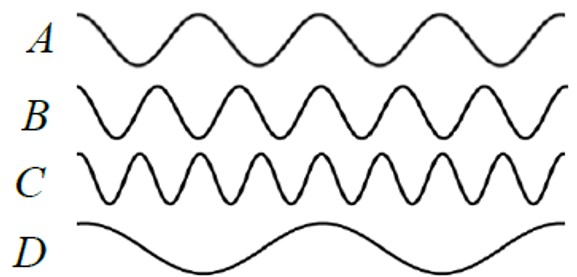
\includegraphics[scale=0.4]{../figs/G11-FINAL-SEM1-001-1}}
	\loigiai{}
\end{ex}
% ===================================================================
\begin{ex}
Gọi $v_{\mathrm{r}}$, $v_{\mathrm{l}}$, $v_{\mathrm{k}}$  lần lượt là tốc độ truyền của sóng dọc trong các môi trường rắn, lỏng, khí. Sắp xếp nào sau đây là đúng?
	\choice
	{$v_{\mathrm{r}}<v_{\mathrm{l}}<v_{\mathrm{k}}$}
	{$v_{\mathrm{l}}<v_{\mathrm{r}}<v_{\mathrm{k}}$}
	{$v_{\mathrm{k}}<v_{\mathrm{r}}<v_{\mathrm{l}}$}
	{\True $v_{\mathrm{k}}<v_{\mathrm{l}}<v_{\mathrm{r}}$}
	\loigiai{}
\end{ex}
% ===================================================================
\begin{ex}
Trong hiện tượng giao thoa sóng mặt nước, người ta quan sát thấy vân giao thoa trung tâm có dạng một đường thẳng và là một vân cực đại. Hai nguồn sóng kết hợp trên mặt nước dao động 
	\choice
	{ngược pha với nhau}
	{vuông pha với nhau}
	{\True cùng pha với nhau}
	{không đồng bộ}
	\loigiai{}
\end{ex}
% ===================================================================
\begin{ex}
	\immini{Cho trạng thái dao động của M trên một phương truyền sóng như hình vẽ. Chiều truyền sóng là
	\choice
	{từ dưới lên trên}
	{từ phải qua trái}
	{từ trên xuống dưới}
	{\True từ trái qua phải}}
	{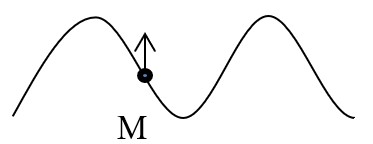
\includegraphics[scale=0.65]{../figs/G11-FINAL-SEM1-001-2}}
	\loigiai{}
\end{ex}
% ===================================================================
\begin{ex}
Bước sóng là khoảng cách giữa hai điểm gần nhau nhất trên phương truyền sóng dao động
	\choice
	{vuông pha với nhau}
	{\True cùng pha với nhau}
	{ngược pha với nhau}
	{lệch nhau về pha}
	\loigiai{}
\end{ex}
% ===================================================================
\begin{ex}
Ở cùng một nơi, con lắc đơn một có chiều dài $\ell_1$ dao động với chu kì $T_1=\SI{2.0}{\second}$ thì con lắc đơn hai có chiều dài $\ell_2=\ell_1/4$ dao động với chu kì là
	\choice
	{$\SI{0.5}{\second}$}
	{$\SI{4.0}{\second}$}
	{\True $\SI{1.0}{\second}$}
	{$\SI{2.0}{\second}$}
	\loigiai{$T=2\pi\sqrt{\dfrac{\ell}{g}}\Rightarrow \dfrac{T^2_2}{T^2_1}=\dfrac{\ell_2}{\ell_1}=\dfrac{1}{4}\Rightarrow T_2=\dfrac{T_1}{2}=\SI{1.0}{\second}$.}
\end{ex}
% ===================================================================
\begin{ex}
Một sóng ngang truyền dọc theo trục $Ox$ với bước sóng $\lambda=\SI{16}{\centi\meter}$. Biên độ sóng là $A=\SI{0.5}{\centi\meter}$ không đổi. Tỉ số giữa tốc độ truyền sóng với tốc độ dao động cực đại của phần tử môi trường là
	\choice
	{$\dfrac{1}{6}$}
	{\True $\dfrac{16}{\pi}$}
	{$\dfrac{\pi}{10}$}
	{$\dfrac{\pi}{4}$}
	\loigiai{$\dfrac{v}{v_{\max}}=\dfrac{\lambda f}{2\pi fA}=\dfrac{\lambda}{2\pi A}=\dfrac{16}{\pi}$.}
\end{ex}
% ===================================================================
\begin{ex}
\immini{Một chất điểm dao động điều hòa theo phương nằm ngang quanh vị trí cân bằng O, với biên độ A. Hình bên là đồ thị biểu diễn sự phụ thuộc của gia tốc tức thời $a$ của chất điểm theo thời gian $t$. Lấy $\pi^2=10$. Phương trình li độ dao động của chất điểm theo thời gian $t$ ($t$ tính bằng giây) là
	\choice
	{$x=\xsi{12,5\cos\left(2\pi t-\dfrac{\pi}{4}\right)}{\centi\meter}$}
	{$x=\xsi{8\cos\left(2,5\pi t+\dfrac{\pi}{4}\right)}{\centi\meter}$}
	{$x=\xsi{12,5\cos\left(2\pi t+\dfrac{\pi}{4}\right)}{\centi\meter}$}
	{\True $x=\xsi{8\cos\left(2,5\pi t-\dfrac{\pi}{4}\right)}{\centi\meter}$}}
{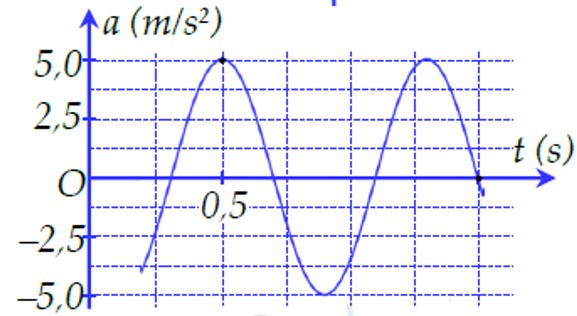
\includegraphics[scale=0.6]{../figs/G11-FINAL-SEM1-001-3}}
	
	\loigiai{$T+\dfrac{T}{4}=\SI{1}{\second}\Rightarrow T=\SI{0.8}{\second}$\\
	$\omega=\dfrac{2\pi}{T}=\xsi{2,5\pi}{\radian/\second}$\\
	$A=\dfrac{a_{\max}}{\omega^2}=\SI{0.08}{\meter}=\SI{8}{\centi\meter}$\\
	$\varphi_{a\left(t=\SI{0.5}{\second}\right)}=\varphi_{0a}+0,5\omega=\xsi{2\pi}{\radian}\Rightarrow \varphi_{0a}=2\pi-0,5\omega=\xsi{\dfrac{3\pi}{4}}{\radian}$\\
	$\varphi_{0x}=\varphi_{0a}-\pi=\xsi{-\dfrac{\pi}{4}}{\radian}$.
	}
\end{ex}
\Closesolutionfile{ans} 
\section{Câu trắc nghiệm đúng/sai} 
\textit{Thí sinh trả lời từ câu 1 đến câu 4. Trong mỗi ý \textbf{a)}, \textbf{b)}, \textbf{c)}, \textbf{d)} ở mỗi câu, thí sinh chọn đúng hoặc sai}
\setcounter{ex}{0}\\
\Opensolutionfile{ans}[ans/G11-FINAL-SEM1-001-TF]
% ===================================================================
\begin{ex}
Một chất điểm dao động điều hoà với tần số $\SI{2}{\hertz}$ và biên độ dao động $\SI{5}{\centi\meter}$. Xét tính đúng sai của các phát biểu sau:
	\choiceTF[t]
	{\True Chu kì dao động của chất điểm là $\SI{0.5}{\second}$}
	{\True Vận tốc cực tiểu của chất điểm là $\xsi{-20\pi}{\centi\meter/\second}$}
	{Tốc độ trung bình của chất điểm trong một chu kỳ là $
	\SI{32}{\centi\meter/\second}$}
	{\True Khi vật có li độ $\SI{4}{\centi\meter}$ thì tốc độ của vật là $v=\xsi{12\pi}{\centi\meter/\second}$}
	\loigiai{
	\begin{itemchoice}
		\itemch Đúng. $T=\dfrac{1}{f}=\SI{0.5}{\second}$.
		\itemch Đúng. $v_{\min}=-\omega A=\xsi{-20\pi}{\centi\meter/\second}$.
		\itemch Sai. $v_{tb}=\dfrac{s}{T}=\dfrac{4A}{T}=\SI{40}{\centi\meter/\second}$.
		\itemch Đúng. $x^2+\dfrac{v^2}{\omega^2}=A^2\Rightarrow v=\xsi{12\pi}{\centi\meter/\second}$.
	\end{itemchoice}
	}
\end{ex}
% ===================================================================
\begin{ex}
Xét tính đúng/sai của các phát biểu sau khi nói về ứng dụng của sóng.
	\choiceTF[t]
	{\True Đàn guitar là một ứng dụng của hiện tượng sóng dừng}
	{\True Đối với các loại nhạc cụ khí, sáo, kèn, khi ta thổi, cột không khí dao động tạo ra sóng giao thoa}
	{\True Điện thoại vừa là thiết bị thu vừa là thiết bị phát sóng điện từ}
	{\True Công nghệ sonar dựa vào sự phản xạ của sóng âm dùng để phát hiện và đo lường khoảng cách của các tàu ngầm hay các vật thể dưới nước}
	\loigiai{}
\end{ex}
% ===================================================================
\begin{ex}
Một người quan sát sóng nước trên mặt hồ thấy khoảng cách giữa hai đỉnh sóng liên tiếp là $\SI{1.5}{\meter}$ và có 6 ngọn sóng lướt qua mặt trong 10 giây.
	\choiceTF[t]
	{Sóng truyền trên mặt hồ là sóng dọc}
	{\True Giá trị của bước sóng là $\SI{1.5}{\meter}$}
	{Chu kì của sóng là $\SI{1.67}{\second}$}
	{Tốc độ truyền sóng trên mặt nước là $\SI{1.5}{\meter/\second}$}
	\loigiai{\begin{itemchoice}
			\itemch Sai. Sóng ngang.
			\itemch Đúng.
			\itemch Sai. $T=\dfrac{t}{N}=\dfrac{10}{5}=\SI{2}{\second}$.
			\itemch Sai. Tốc độ truyền sóng $v=\dfrac{\lambda}{T}=\dfrac{1,5}{2}=\SI{0.75}{\meter/\second}$.
	\end{itemchoice}}
\end{ex}
% ===================================================================
\begin{ex}
Loa nghe nhạc là một thiết bị biến đổi tín hiệu điện thành dao động cơ học để tái tạo âm thanh nhờ sự dao động của màng loa. Một loa nghe biết màng loa rung theo tín hiệu dao động điều hòa với tần số $\SI{500}{\hertz}$ và có độ rời cực đại của tâm màng loa là $\SI{3}{\milli\meter}$. Lấy $\pi^2=10$. Xét tính đúng sai của các phát biểu sau:
	\choiceTF[t]
	{\True Chu kì dao động của màng loa là $\SI{0.002}{\second}$}
	{\True Tâm màng loa dao động trên quỹ đạo dài $\SI{3}{\milli\meter}$}
	{Vận tốc dao động cực đại của tâm màng loa là $\xsi{3\pi}{\meter/\second}$}
	{Gia tốc dao động cực tiểu của tâm màng loa là $\SI{0}{\milli\meter/\second^2}$}
	\loigiai{\begin{itemchoice}
			\itemch Đúng.
			\itemch Đúng.
			\itemch Sai. $v_{\max}=\omega A=2\pi f A=\xsi{1,5\pi}{\meter/\second}$.
			\itemch Sai. $a_{\min}=-\omega^2A\neq 0$.
	\end{itemchoice}}
\end{ex}
\Closesolutionfile{ans}
\section{Câu trắc nghiệm trả lời ngắn} \textit{Thí sinh trả lời từ câu 1 đến câu 6}
\setcounter{ex}{0}
\Opensolutionfile{ans}[ans/G11-FINAL-SEM1-001-TL]
% ===============================================================
\begin{ex}
Trong thí nghiệm Young về giao thoa ánh sáng, nguồn phát bức xạ đơn sắc có bước sóng $\SI{500}{\nano\meter}$, khoảng cách giữa hai khe là $\SI{1.5}{\milli\meter}$, màn quan sát cách mặt phẳng hai khe $\SI{2.4}{\meter}$. Khoảng vân quan sát được bằng bao nhiêu milli mét $\left(\si{\milli\meter}\right)$? 
	\shortans[oly]{0,8}
	\loigiai{
		$i=\dfrac{\lambda D}{a}=\SI{0.8}{\milli\meter}$.
	}
\end{ex}
% ===============================================================
\begin{ex}
Xét sóng truyền trên mặt nước có bước sóng $\SI{48}{\centi\meter}$. Hai điểm trên cùng một phương truyền sóng dao động lệch pha nhau $\xsi{\dfrac{\pi}{6}}{\radian}$. Hai điểm này cách nhau một đoạn bằng bao nhiêu $\si{\centi\meter}$?
	\shortans[oly]{4}
	\loigiai{
		$\Delta \varphi=\dfrac{2\pi d}{\lambda}\Rightarrow d=\SI{4}{\centi\meter}$.
	}
\end{ex}
% ===============================================================
\begin{ex}
Trên một sợi dây đàn hồi AB dài $\SI{60}{\centi\meter}$ đang có sóng dừng với hai đầu A và B cố định. Quan sát trên dây AB có 3 bụng sóng. Tốc độ truyền sóng trên dây là $\SI{4}{\meter/\second}$ thì tần số sóng trên dây bằng bao nhiêu hertz $\left(\si{\hertz}\right)$? 
	\shortans[oly]{10}
	\loigiai{
		$f=\dfrac{nv}{2\ell}=\SI{10}{\hertz}$.
	}
\end{ex}
% ===============================================================
\begin{ex}
	\immini{Một chất điểm đang dao động điều hòa trên phương nằm ngang, có đồ thị biểu diễn sự phụ thuộc của vận tốc tức thời $v$ theo thời gian $t$ như hình vẽ bên. Gia tốc cực đại của chất điểm là bao nhiêu $\si{\meter/\second^2}$. Lấy $\pi^2=10$.}
	{\vspace{-0.5cm}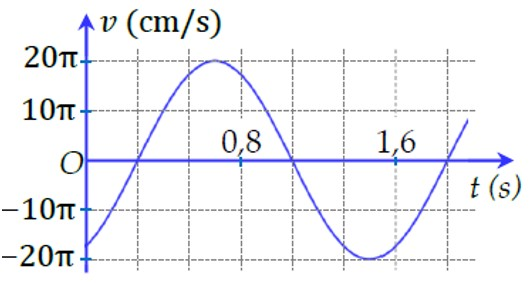
\includegraphics[scale=0.5]{../figs/G11-FINAL-SEM1-001-4}}
	\shortans[oly]{2,5}
	\loigiai{
		$T=\SI{1.6}{\second}$.\\
		$a_{\max}=\omega v_{\max}=\SI{2.5}{\meter/\second^2}$.
	}
\end{ex}
% ===============================================================
\begin{ex}
Thực hiện thí nghiệm giao thoa sóng trên mặt nước với hai nguồn kết hợp đặt tại A và B cách nhau $\SI{20}{\centi\meter}$, dao động cùng pha theo phương thẳng đứng, phát ra hai sóng lan truyền có bước sóng $\SI{3.5}{\centi\meter}$. Trên mặt nước, tổng số dãy dao động với biên độ cực đại là bao nhiêu? 
	\shortans[oly]{11}
	\loigiai{
		$\dfrac{-20}{3,5}\le k\le \dfrac{20}{3,5}\Leftrightarrow -5,7\le k\le 5,7\Rightarrow N_{\max}=11$.
	}
\end{ex}
% ===============================================================
\begin{ex}
\immini{Một nhóm học sinh thực hiện thí nghiệm giao thoa khe Young để xác định bước sóng của chùm tia laser. Khoảng cách giữa hai khe hẹp là $\SI{0.15}{\milli\meter}$ và khoảng cách từ hai khe đến màn là $\SI{80}{\centi\meter}$. Vị trí các vân sáng, vân tối được đánh dấu trên tờ giấy trắng như hình vẽ. Dùng thước cặp đo được khoảng cách $L=\SI{14}{\milli\meter}$. Bước sóng ánh sáng trong thí nghiệm bằng bao nhiêu nano mét $\left(\si{\nano\meter}\right)$? \textit{(Kết quả Làm tròn đến chữ số hàng đơn vị)}}
{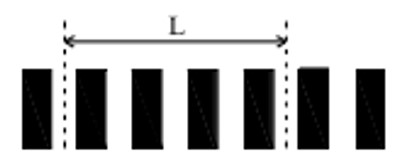
\includegraphics[scale=0.5]{../figs/G11-FINAL-SEM1-001-5}}
	\shortans[oly]{656}
	\loigiai{
		$i=\dfrac{L}{4}=\SI{3.5}{\milli\meter}$.\\
		$\lambda=\dfrac{ia}{D}=\SI{656.25}{\nano\meter}$.
	}
\end{ex}
\Closesolutionfile{ans}
\begin{center}
	\textbf{--- HẾT ---}
\end{center}